%!TEX root = ../report.tex
\section{Stories and use-cases}
In figure \ref{fig:usecase-diagram} is the use-case diagram displayed. This provides an overview of the use-cases with their actors.

\begin{figure}[h]
\centering
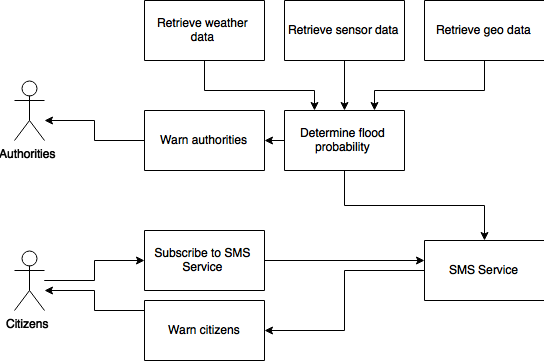
\includegraphics[width=90mm]{images/usecaseDiagram.png}
\caption{Use-case diagram}
\label{fig:usecase-diagram}
\end{figure}

\subsection{A citizen receives a warning about an upcoming flood}
\textbf{Scope:} Warning part of the system\\\\
\textbf{Level:} Main process\\\\
\textbf{Primary actor:} Citizen\\\\
\textbf{Stakeholders and interests:}\\

%slides say:
%	Name & \\
%	Number & \\
%	Primary actor &  \\
%	Scope &  \\
%	Level &  \\
%	Extensions &  \\
%	Sub-variations & \\

\pgfplotstabletypeset[%
UCTable
]{%
	value & description \\
	Number & \req{uc}\\
	Name & Warn citizens\\%A citizen receives a warning about an upcoming flood \\
	Description & Citizens will be warned in case of a flood \\	
	Stakeholders and interests & \compactList{itemize}{
			\item \textbf{Citizens}: Citizens want to be warned when a flood happens}\\
	Primary actor & Citizen\\
	Scope & Warning part of the system \\
	Level & Main process\\
	Precondition & There is an upcoming flood, the citizens are not warned and they are subscribed to our warning service. \\
	Main success scenario & \compactList{enumerate}{%
			\item Sensors send the data to the processing unit%
			\item The processing unit determines there is an imminent flood%
			\item The processing unit generates a map with vulnerable areas
			\item Text messages containing a warning are send to all subscribers in the vulnerable area
			\item The subscribed citizens receive the warning message }\\
	Postcondition & There is an upcoming flood and the citizens are warned \\
	Extensions & \compactList{itemize}{%
			\item[2a.] Flood doesn't get to dangerous, it retreats. No warning mechanism is triggered
			\item[4a.] The citizen is not in the vulnerable area. No text message is send}\\
	%Sub-variations & \\
}

\pgfplotstabletypeset[%
UCTable
]{%
	value & description \\
	Number & \req{uc}\\
	Name & Warn authorities\\
	Description & Government and emergency services receive a warning about an upcoming flood\\
	Stakeholders and interests & \compactList{itemize}{%
			\item \textbf{Government}: The government wants to warn the citizens in case of a flood
			\item \textbf{Emergency services}: The emergency services want to help the citizens in times of need}\\
	Primary actor & Government, Emergency services\\
	Scope & Warning part of the system \\
	Level & Main process\\
	Precondition & There is an upcoming flood\\
	Main success scenario & \compactList{enumerate}{
			\item The sensors send their data to the processing unit
			\item The processing unit determines there is an upcoming flood
			\item The processing unit generates a range of vulnerable locations
			\item A warning containing the locations is send to the government and the emergency services
			\item The Government and emergency services receive the warning message
			\item The system receives a confirmation that the government and the emergency services received the warning }\\
	Postcondition & There is an upcoming flood and the government and emergency services are warned \\
	Extensions & \compactList{itemize}{%
			\item[2a.] The flood doesn't get to dangerous, it retreats. No warning mechanism is triggered
			\item[6a.] No confirmation is received within 15 seconds. Send warning message in another way}\\
	%Sub-variations & \\
}

%\todo{joris: "The sensors send their data to the processing unit" is removed here, but is the first mss item in the preview usecases}
\pgfplotstabletypeset[%
UCTable
]{%
	value & description \\
	Number & \req{uc}\\
	Name & Guide citizens\\
	Description & A citizen requests guidance to get to a safe place in a flooded area \\
	Stakeholders and interests & \compactList{itemize}{%
			\item \textbf{Citizens}: Citizens want to be guided to a safe place in case of a flood
			\item \textbf{Emergency services}: The emergency services want to help the citizens in times of need}\\
	Primary actor & Citizen\\
	Scope & Guidance part of the system \\
	Level & Main process\\
	Precondition & There is a flood and the citizen is subscribed to the warning service. \\
	Main success scenario & \compactList{enumerate}{%
			\item The processing unit determined there is a flood%
			\item The processing unit determines generic routes
			\item The processing unit turns this routes into a MMS message with the right directions
			\item The generic routes are send through MMS message to all subscribed phone numbers}\\
	Postcondition & Citizen received his/her personal route to safety \\
	Extensions & \compactList{itemize}{%
			\item[4a.] MMS message can't be send. Wait a minute and try to resend}\\
	%Sub-variations & \\
}

\pgfplotstabletypeset[%
UCTable
]{%
	value & description \\
	Number & \req{uc}\\
	Name & Retrieve weather data\\%A citizen receives a warning about an upcoming flood \\
	Description & The system receives data from the weather forecast service \\
	Stakeholders and interests & \compactList{itemize}{%
			\item \textbf{Developers}: Developers would like to have a simple to use API}\\
	Primary actor & Developers\\
	Scope & Monitoring part of the system \\
	Level & Main process\\
	Precondition & The system needs external weather data to predict floods \\
	Main success scenario & \compactList{enumerate}{%
			\item The processing unit determines it needs forecast weather data%
			\item A call is made to the weather forecast service%
			\item The weather forecast service returns the requested data}\\
	Postcondition & The system received the forecast data \\
	Extensions & \compactList{itemize}{%
			\item[3a.] The data can't be returned. Repeat this process with another weather forecast service. If none are available, proceed monitoring without weather forecast data. After 5 minutes try to reconnect.}\\
	%Sub-variations & \\
}
%If we decide to use user input
% \subsection{A citizen reports an obstruction}
% \textbf{Scope:} Monitoring part of the system\\\\
% \textbf{Level:} Main process\\\\
% \textbf{Primary actor:} Citizen\\\\
% \textbf{Stakeholders and interests:}\\
% 	1. Citizen - A citizen wants to report an obstruction to make the guidance part more reliable. \\\\
% \textbf{Preconditions:} There is an obstruction which is not yet reported. \\
% \textbf{Postconditions:} There is an obstruction which is reported by a citizen and is known in the system. \\\\
% \textbf{Main succes scenario:} \\
% 1 - There is an obstruction somewhere in the area. \\
% 2 - The citizen opens our application on his smartphone. \\
% 3 - The citizen reports the kind of obstruction and the location. \\
% 4 - The system gets the obstruction information as input. \\
% 5 - The obstruction is processed in the system and visible to other citizens. \\\\
% \textbf{Extensions:} \\
% 3a - The citizen doesn't know the location, GPS can be used in this case. If GPS doesn't work, the obstruction can't be reported. \\
% 4a - The smartphone can't send the information. In this case, the obstruciton can't be reported. 
